\appendix
\chapter*{Annexes}
\addcontentsline{toc}{chapter}{Annexes}
\renewcommand{\thesection}{\Alph{section}}
\section{Discussion du débit binaire près de l'ascenceur}
\label{discussion-debit-critique}
Th{\'e}oriquement, on devrait observer un blocage total du signal dans cette
zone en raison des mat{\'e}riaux utilis{\'e}s. 

Cependant, nous avons
rencontr{\'e} un probl{\`e}me inattendu de valeur de puissance trop
{\'e}lev{\'e}e (par exemple autour de $- 68 \mathrm{dBm}$ pour une station de base en $(9.4,
7) m$ avec $20 \mathrm{dBm}$ de puissance d'{\'e}mission).\\

Nous avons tent{\'e} de le
r{\'e}soudre de plusieurs mani{\`e}res. 
Nous avons d{\'e}plac{\'e} les murs
pour v{\'e}rifier s'il y avait un probl{\`e}me au niveau des coins. 
Nous avons
v{\'e}rifi{\'e} avec notre fonction \textit{Rays to Single Cell}, les rayons
trac{\'e}s {\`a} cet endroit. Nous avons compar{\'e} et cherch{\'e} l'erreur
avec des camarades, {\`a} plusieurs reprises et pendant longtemps, sans
succ{\`e}s. Plusieurs mat{\'e}riaux ont {\'e}t{\'e} test{\'e}s, et nous avons
v{\'e}rifi{\'e} les propri{\'e}t{\'e}s physiques des murs {\`a} de nombreuses
reprises. 
\\
En outre, nous avons rev{\'e}rifi{\'e} toutes les fonctions de
calcul des coefficients et r{\'e}{\'e}crit plusieurs parties du code plusieurs
fois dans l'espoir de trouver la faille. Enfin, diff{\'e}rentes positions de
la station de base et plusieurs stations ont {\'e}t{\'e} test{\'e}es.
\\ 
Malgr{\'e} tous ces efforts, le probl{\`e}me persiste et reste un point
d'investigation pour des travaux futurs. 


Ce qui reste {\'e}trange tout de même, est que
c'est la seule zone dans laquelle une si grande erreur de d{\'e}bit binaire
persiste. 

\begin{figure}[H]
    \centering
    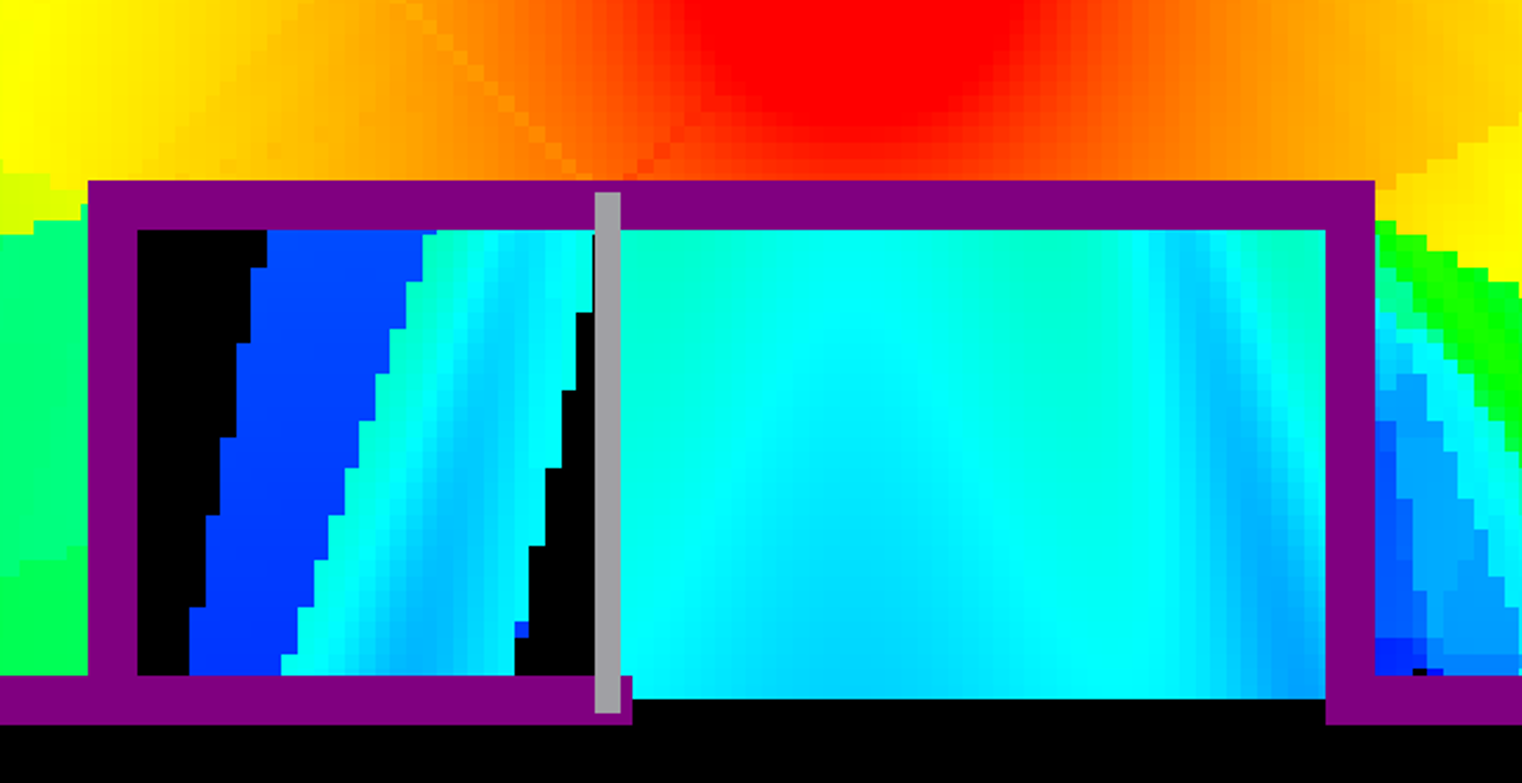
\includegraphics[width=0.8\textwidth]{latex/images/bug-ascenseur.png}
    \label{fig:bug-ascenseur}
\end{figure}

\begin{figure}[H]
    \centering
    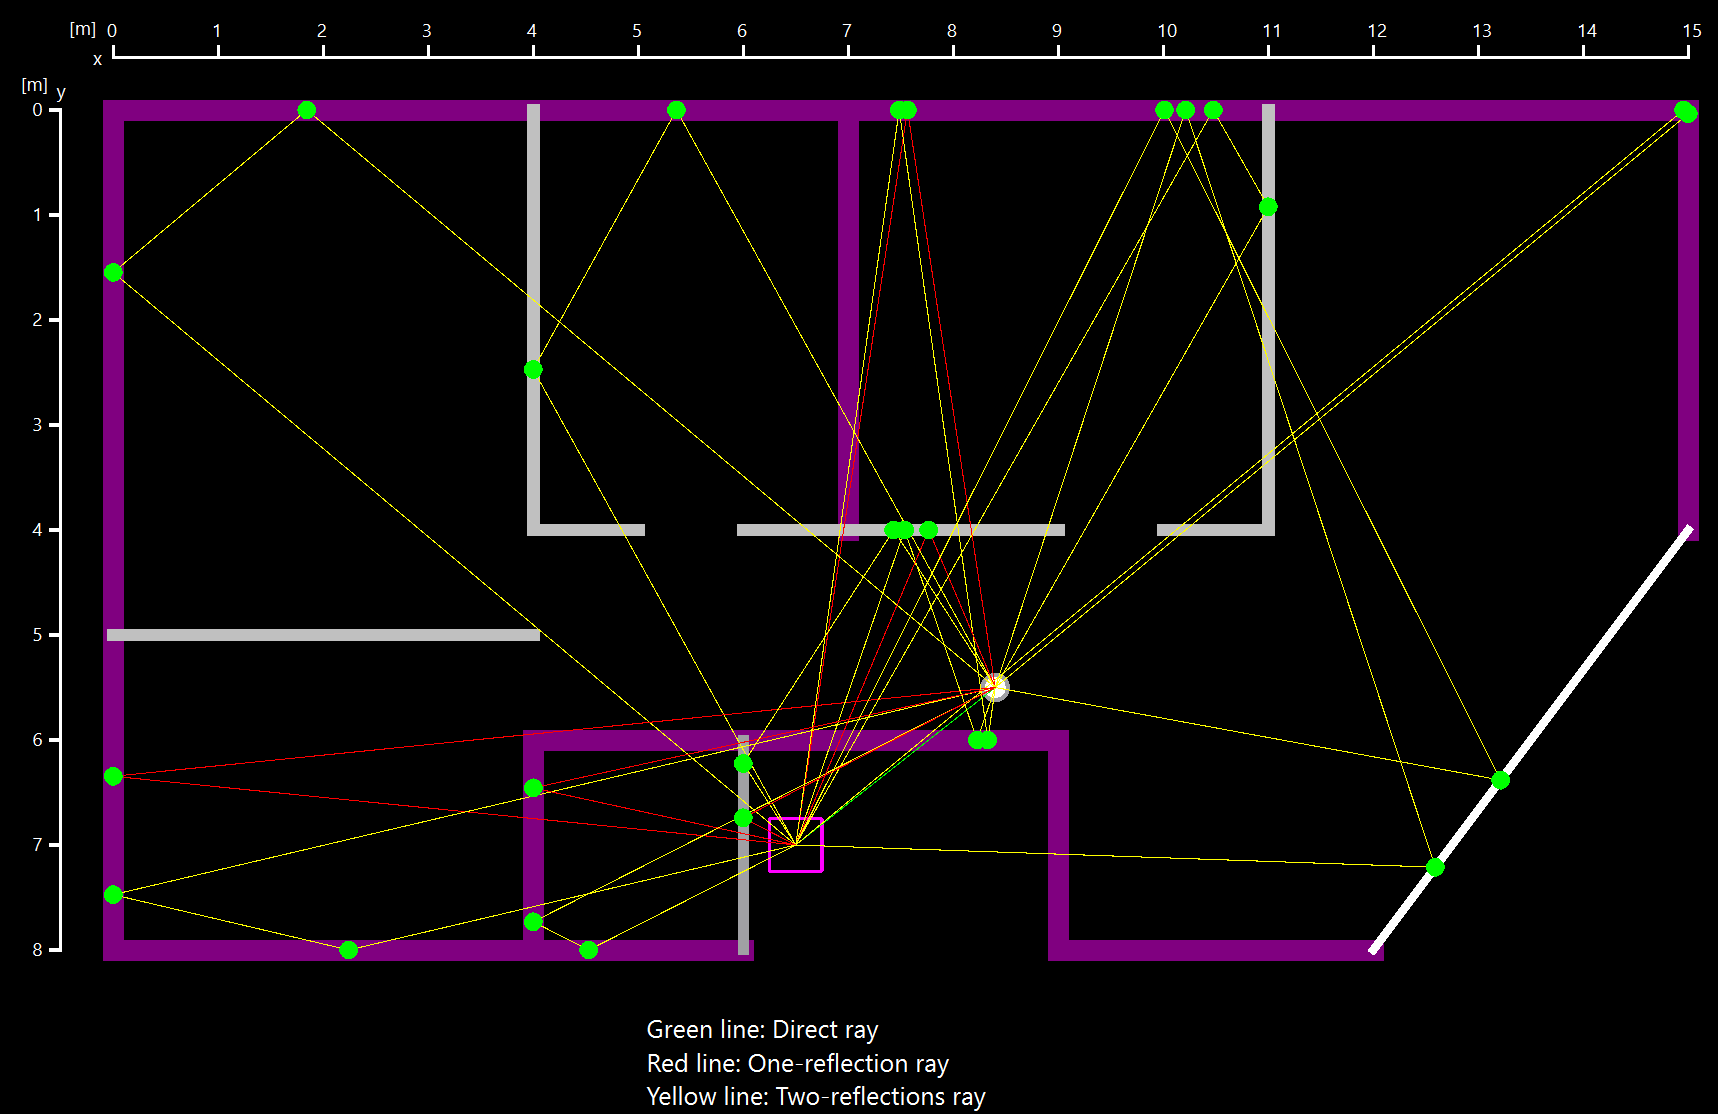
\includegraphics[width=\textwidth]{latex/images/bug-ascenseur-rays.png}
    \label{fig:bug-ascenseur-rays}
\end{figure}

\newpage
\section{Code}
Cette partie de l'annexe comprend la quasi-totalité du code du projet.
%\usemintedstyle{pastie}
\subsection{main.cpp}
\label{appendix:main.cpp}

Lance simplement l'interface utilisateur de l'aplication.

\inputminted[
frame=lines,
framesep=2mm,
baselinestretch=1.2,
fontsize=\footnotesize,
linenos,
breaklines
]{cpp}{../main.cpp}

% \begin{minted}[
% frame=lines,
% framesep=2mm,
% baselinestretch=1.2,
% fontsize=\footnotesize,
% linenos
% ]{python}

% for i in range(5):
%     print(i) # oui

% \end{minted}


\newpage
\subsection{simulation.cpp}
\label{appendix:simulation.cpp}
Ce fichier contient toute l'implémentation de la logique de la simulation.\\
Le \textit{header file \textbf{.h}} définissant la classe \textbf{Simulation} se trouve dans le \underline{\href{https://github.com/LucasPlacentino/802_11ay-Raytracing-Simulator}{Github}} du projet.
\inputminted[
frame=lines,
framesep=2mm,
baselinestretch=1.2,
fontsize=\footnotesize,
linenos,
breaklines
]{cpp}{../simulation.cpp}

\newpage
\subsection{transmitter.cpp}
\label{appendix:transmitter.cpp}
Ce fichier contient toute l'implémentation de la classe \textbf{Transmitter}.\\
Le \textit{header file \textbf{.h}} définissant la classe \textbf{Transmitter} se trouve dans le \underline{\href{https://github.com/LucasPlacentino/802_11ay-Raytracing-Simulator}{Github}} du projet.
\inputminted[
frame=lines,
framesep=2mm,
baselinestretch=1.2,
fontsize=\footnotesize,
linenos,
breaklines
]{cpp}{../transmitter.cpp}

\newpage
\subsection{receiver.cpp}
\label{appendix:receiver.cpp}
Ce fichier contient toute l'implémentation de la classe \textbf{Receiver}.\\
Le \textit{header file \textbf{.h}} définissant la classe \textbf{Receiver} se trouve dans le \underline{\href{https://github.com/LucasPlacentino/802_11ay-Raytracing-Simulator}{Github}} du projet.
\inputminted[
frame=lines,
framesep=2mm,
baselinestretch=1.2,
fontsize=\footnotesize,
linenos,
breaklines
]{cpp}{../receiver.cpp}

\newpage
\subsection{obstacle.cpp}
\label{appendix:obstacle.cpp}
Ce fichier contient toute l'implémentation de la classe \textbf{Obstacle} pour les murs.\\
Le \textit{header file \textbf{.h}} définissant la classe \textbf{Obstacle} se trouve dans le \underline{\href{https://github.com/LucasPlacentino/802_11ay-Raytracing-Simulator}{Github}} du projet.
\inputminted[
frame=lines,
framesep=2mm,
baselinestretch=1.2,
fontsize=\footnotesize,
linenos,
breaklines
]{cpp}{../obstacle.cpp}

\newpage
\subsection{ray.cpp}
\label{appendix:ray.cpp}
Ce fichier contient toute l'implémentation de la classe \textbf{Ray}.\\
Le \textit{header file \textbf{.h}} définissant la classe \textbf{Ray} se trouve dans le \underline{\href{https://github.com/LucasPlacentino/802_11ay-Raytracing-Simulator}{Github}} du projet.
\inputminted[
frame=lines,
framesep=2mm,
baselinestretch=1.2,
fontsize=\footnotesize,
linenos,
breaklines
]{cpp}{../ray.cpp}

\newpage
\subsection{raysegment.cpp}
\label{appendix:raysegment.cpp}
Ce fichier contient toute l'implémentation de la classe \textbf{RaySegment}.\\
Le \textit{header file \textbf{.h}} définissant la classe \textbf{RaySegment} se trouve dans le \underline{\href{https://github.com/LucasPlacentino/802_11ay-Raytracing-Simulator}{Github}} du projet.
\inputminted[
frame=lines,
framesep=2mm,
baselinestretch=1.2,
fontsize=\footnotesize,
linenos,
breaklines
]{cpp}{../raysegment.cpp}

\newpage
\subsection{parameters.h}
\label{appendix:parameters.h}
Ce fichier contient les paramètres de la simulation à définir lors de la compilation.
\inputminted[
frame=lines,
framesep=2mm,
baselinestretch=1.2,
fontsize=\footnotesize,
linenos,
breaklines
]{cpp}{../parameters.h}

% ---- pas nécessaire d'afficher mainwindow.cpp ? ----
%\newpage
%\section{mainwindow.cpp}
%\label{appendix:mainwindow.cpp}
%
%\inputminted[
%frame=lines,
%framesep=2mm,
%baselinestretch=1.2,
%fontsize=\footnotesize,
%linenos,
%breaklines
%]{cpp}{../mainwindow.cpp}

\newpage
\subsection{algorithme.cpp}
\label{appendix:algorithme.cpp}
Ce fichier contient l'implémentation de l'algorithme d'optimisation de placement optimal de station de base, selon la moyenne des puissances de chaque cellule la plus haute, et selon le minimum de cellule en dessous du seuil pour un débit binaire minimum.
\inputminted[
frame=lines,
framesep=2mm,
baselinestretch=1.2,
fontsize=\footnotesize,
linenos,
breaklines
]{cpp}{../algorithme.cpp}

\newpage
\subsection{Autres parties du code}
\label{appendix:autres-codes}
D'autres parties du code sont disponibles sur le Github du projet:\\
\underline{\url{https://github.com/LucasPlacentino/802_11ay-Raytracing-Simulator}}.\\

Ceci inclut:
\begin{itemize}
    \item \textbf{mainwindow.cpp} (et son \textbf{.h}) : classe s'occupant de l'interface utilisateur.
    \item \textbf{tp4.cpp} : code reprenant l'implémentation de la simulation exclusivement utilisée pour le TP4, qui a servi de base initiale avant d'étendre les fonctionnalités au projet global.
    \item \textbf{CMakeLists.txt} : le CMake généré et utilisé par \textit{QtCreator}.
\end{itemize}
